\documentclass[french]{book}
\usepackage{teach}
\usepackage{verbatim}
%\usepackage[french]{babel}

%%% Couleurs
\redefinecolor{thm}{title}{bgcolor}{alizarin}
\redefinecolor{prop}{title}{bgcolor}{meatbrown}
\redefinecolor{defn}{title}{bgcolor}{olivine}
\definecolor{alizarin}{rgb}{0.82, 0.1, 0.26}
\definecolor{meatbrown}{rgb}{0.9, 0.72, 0.23}
\definecolor{olivine}{rgb}{0.6, 0.73, 0.45}
%%% Les symboles
\usepackage{amsmath}
\usepackage{amssymb}
\usepackage{amsfonts}
\usepackage{amsthm}
\usepackage{mwe}
\usepackage{yhmath} 
%%% Ensemble de nombre
\newcommand{\R}{\mathbb{R}}
%\newcommand{\C}{\mathds {C}}
\newcommand{\N}{\mathbb{N}}
\newcommand{\Z}{\mathbb{Z}}
\newcommand{\Q}{\mathbb{Q}}
\newcommand{\D}{\mathbb{D}}
%%% Tableau
\usepackage{array}
\usepackage{multicol}
\setlength{\multicolsep}{3pt}
%%% Figures
\usepackage{graphicx}
\graphicspath{{Figures/}}
%%% Affichage 
\newcommand{\ds}{\displaystyle}
%%% Tableau
\usepackage{tikz}
\usepackage{tkz-tab}
%%% Lecon creuse/pleine
\usepackage{dashundergaps}
%\TeacherModeOff
\TeacherModeOn
\newcommand{\mgap}[1]{\text{\gap*[b]{\ensuremath{#1}}}} %dashundergaps math mode
%%% Table des matières
%\tableofcontents 
\setcounter{chapter}{5}


\begin{document}
\chapter{Logarithme décimal}
\section{Définitions et généralités sur le logarithme décimal}

\begin{defn}
Soit $y \in \mgap{\mathbb{R}_+^*}$ tel que: 
$$y=10^x$$
alors il existe $x \in \mathbb{R}$ \gap*{unique} et tel que : $$x:=log(y)$$ 
\end{defn}

\begin{exemple}
$$log(100)=log(10^2)=2 \qquad log(1)=log(10^0)=0 \qquad log(0,0001)=log(10^{-4})=-4 \qquad log(543)\approx 2,73  $$
\end{exemple}

\begin{rem}
Attention le logarithme décimal d'un \gap*{nombre négatif ou nul} n'existe pas.
\end{rem}

\begin{defn}
$log$ est une fonction appelée logarithme décimale définie comme ci-dessous
$$log: \mathbb{R}^*_+ \longrightarrow \mathbb{R}$$
$$ \qquad \quad x \mapsto log(x) $$ 
\end{defn}

\includegraphics[scale=0.7]{log.1}

\section{Variations et signes du logarithme décimal}

\begin{prop}
La fonction $log$ est une fonction \gap*{strictement croissante} sur $\mathbb{R}_+^*$, autrement dit, cette fonction \gap*{conserve l'ordre}.
\end{prop}

\begin{exemple}
On sait que $10<51<100$ donc $log(10)<log(51)<log(100)$ autrement dit $1<log(51)<2$.
\end{exemple}

\begin{prop}
La fonction $log$ admet le tableau de signe suivant sur $\mathbb{R}_+^*$
\begin{center}
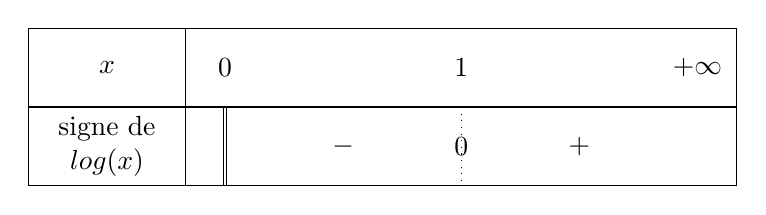
\begin{tikzpicture}
   \tkzTabInit{$x$ / 1 , \text{signe de} $log(x)$ / 1}{$0$, $1$, $+\infty$}
   \tkzTabLine{d, - , z, +, }
\end{tikzpicture}
\end{center}
\end{prop}

\section{Relation fonctionnelle et propriétés algébriques}
\begin{thm*}[Relation fonctionnelle]
Pour tout $a,b \in \mathbb{R}_+^*$ on a
 $$log(a)+log(b)=log(a\times b)$$
\end{thm*}

\begin{rem}
On remarque que \gap*{la somme des logarithmes} est égale au \gap*{logarithme du produit}.\\

En particulier, on voit le lien avec un théorème sur les fonctions exponentielles déjà vu, \textit{le produits des exponentielles est égale à l'exponentielle de la somme}.
\end{rem}

\begin{cor*}[Propriétés algébriques]
\begin{multicols}{3}
\begin{itemize}
\item $log(\dfrac{1}{b})=-log(b)$
\item $log(\dfrac{a}{b})	=log(a)-log(b)$
\item $log(a^b)=blog(a)$
\end{itemize}
\end{multicols}
\end{cor*}

\begin{exemple}
\begin{multicols}{3}
\begin{itemize}
\item $log(\dfrac{1}{5})=\mgap{-log(5)}$
\item $log(\dfrac{4}{7})=\mgap{log(4)-log(7)}$
\item $log(5^7)=\mgap{7log(5)}$
\end{itemize}
\end{multicols}
\end{exemple}

\newpage

\section{Exercices}
\begin{exocor}
Résoudre les équations et inéquation suivantes:
\begin{multicols}{4}
\begin{enumerate}
\item $2^x=100$
\item $x^{4,5}=13$
\item $2000 \times 1,4^x=10000$ 
\item $30 x^{21}=500$ 
\item $5^x < 0,0001$ 
\item $ x^{7,1}>10000$
\item $5 \times 2^x > 500$
\item $400 \times x^{0,5}< 100$

\end{enumerate}
\end{multicols}
\end{exocor}

\begin{exocor}

\begin{enumerate}
\item Exprimer les quantités suivantes en fonction de $log(3)$
\begin{multicols}{3}
\begin{enumerate}
\item $log(300)$
\item $log(3000)$
\item $log(27)$
\item $log(0,09)$
\item $log(0,0081)$
\item $log(0,3)$
\end{enumerate}
\end{multicols}

\item Exprimer les quantités suivantes en fonction de $log(3)$ et/ou $log(2)$.

\begin{multicols}{3}
\begin{enumerate}
\item $log(\dfrac{1}{2})$
\item $log(54)$
\item $log(\dfrac{9}{8})$
\end{enumerate}
\end{multicols}


\item Exprimer les quantités suivantes en fonction de $log(a)$ avec $a \in \mathbb{R}_+^*$.

\begin{multicols}{3}
\begin{enumerate}
\item $log(7a^3)$
\item $log(\dfrac{3a^2}{a^5})$
\item $log(1000a^3)$
\end{enumerate}
\end{multicols}
\end{enumerate}
\end{exocor}


\begin{exocor}
L'échelle de Richter est une échelle permettant le classement de la puissance d'une secousse sismique, dont les magnitudes sont comprises sur l'intervalle $[0;10]$. La magnitudes de Richter est calculé de la manière suivante 
$$M=log(A)-log(A_0)$$
Avec $M$ représentant la magnitude et où $A$ représente l’amplitude maximale relevée par le sismographe et $A_0$ une amplitude de référence. 
\begin{enumerate}
\item Calculer la magnitude d'un séisme si $A=A_0$, $A=100 \times A_0$, $A=10000 \times A_0$.
\item La magnitude connue la plus importante est de $9,5$. Elle a été enregistrée au Chili en mai 1960. déterminer $\dfrac{A}{A_0}$.
\item Un pays vient de connaître un séisme de magnitude 8 suivi d’une réplique de magnitude 4. Un journaliste écrit alors que la réplique a été deux fois moins puissante que le premier séisme. Que pensez-vous de cette affirmation du journaliste ? Justifier votre réponse.
\end{enumerate}
\end{exocor}

\begin{exocor}
Le nombre de bactérie au sein d'un être vivant est modéliser par la fonction $b$ définie sur $\mathbb{R}_+^*$ telle que $b(t)=15000 \times (1,343)^t$ avec $t$ exprimé en heure.

\begin{enumerate}
\item Que cherche t-on à savoir quand on résout l'inéquation $b(t)>50000$ ?
\item Résoudre l'inéquation $b(t)>50000$ et conclure par une phrase faisant le lien avec le problème donné.
\end{enumerate} 
\end{exocor}

\begin{exocor}
Monsieur Truque souhaite se constituer une épargne en plaçant une certaine somme d'argent sur un
compte rémunéré bloqué. Pour savoir quand son objectif sera atteint, il doit résoudre l'inéquation
$$800 \times (1,025)^n > 1200$$

Déterminer l'objectif de Monsieur Truque, les modalités de son placement puis résoudre le problème.
\end{exocor}
\newpage
%%Corrigé%%

\section{Corrigés}

\begin{corrige}
\begin{enumerate}
\item $2^x=100 \Longleftrightarrow log(2^x)=log(100) \Longleftrightarrow xlog(2)=2 \Longleftrightarrow x=\dfrac{2}{log(2)}$
\item $x^{4,5}=13 \Longleftrightarrow  x=13^{\frac{1}{4,5}}$
\item $2000 \times 1,4^x=10000 \Longleftrightarrow 1,4^x=\dfrac{10000}{2000} \Longleftrightarrow 1,4^x= 5 \Longleftrightarrow log(1,4^x)=log(5) \Longleftrightarrow xlog(1,4)=log(5)\Longleftrightarrow x=\dfrac{log(5)}{log(1,4)}$
\item $30 x^{21}=500 \Longleftrightarrow x^{21}=\dfrac{500}{30} \Longleftrightarrow x = (\dfrac{50}{3})^{\dfrac{1}{21}}$
\item $5^x < 0,0001 \Longleftrightarrow log(5^x) < log(0,0001) \Longleftrightarrow xlog(5)<-4 \Longleftrightarrow x< -\dfrac{4}{log(5)}$
\item $ x^{7,1}>10000 \Longleftrightarrow x > 10000^{\dfrac{1}{7,1}}$
\item $5 \times 2^x > 500 \Longleftrightarrow 2^x > 100 \Longleftrightarrow log(2^x)>log(100) \Longleftrightarrow xlog(2)>2 \Longleftrightarrow x> \dfrac{2}{log(2)}$
\item  $400 \times x^{0,5}< 100 \Longleftrightarrow x^{0,5} < \dfrac{1}{4} \Longleftrightarrow 0< x < (\dfrac{1}{4})^{\dfrac{1}{0.5}}  \Longleftrightarrow 0<x< \dfrac{1}{16}$

\end{enumerate}
\end{corrige}

\begin{corrige}
\begin{enumerate}
\item 
\begin{multicols}{2}
\begin{enumerate}[label=\textbf{\alph*.}]
\item $log(300)=log(3)+log(100)=2+log(3)$
\item $log(3000)=log(3)+3$
\item $log(27)=log(3^3)=3log(3)$
\item $log(0,09)=log(3^2 \times 10^{-2})=2log(3)-2$
\item $log(0,0081)=log(3^4 \times 10^{-4})=4log(3)-4$
\item $log(0,3)=log(3\times 10^{-1})$
\end{enumerate}
\end{multicols}
\item
\begin{enumerate}[label=\textbf{\alph*.}]
\item $log(\dfrac{1}{2})=-log(2)$
\item $log(54)=log(27\times 2)=log(3^3\times 2)=3log(3)+log(2)$
\item $log(\dfrac{9}{8})=log(9)-log(8)=2log(3)-3log(2)$
\end{enumerate}
\item
\begin{enumerate}[label=\textbf{\alph*.}]
\item $log(7a^3)=log(7)+3log(a)$
\item $log(\dfrac{3a^2}{a^5})=log(3)+2log(a)-5log(a)$
\item $log(1000a^3)=3+3log(a)$
\end{enumerate}
\end{enumerate}

\end{corrige}

\begin{corrige}
\begin{enumerate}
\item Calculer la magnitude d'un séisme si $A=A_0$, $A=100 \times A_0$, $A=10000 \times A_0$.
$$M=0, \qquad M=2, \qquad M=4 $$

\item La magnitude connue la plus importante est de $9,5$. Elle a été enregistrée au Chili en mai 1960. Déterminer $\dfrac{A}{A_0}$
$$log(A)-log(A_0)=9,5$$
$$\Longleftrightarrow log(\dfrac{A}{A_0})=9,5$$
$$\Longleftrightarrow \dfrac{A}{A_0}=10^{9,5}$$
$$\Longrightarrow \dfrac{A}{A_0}\approx 3162277660$$

\item Un pays vient de connaître un séisme de magnitude 8 suivi d’une réplique de magnitude 4. Un journaliste écrit alors que l'amplitude de la réplique a été deux fois moins puissante que l'amplitude premier séisme. Que pensez-vous de cette affirmation du journaliste ? Justifier votre réponse.
$$M_1=8 \Longleftrightarrow log(\dfrac{A_1}{A_0})= 8 \Longleftrightarrow \dfrac{A_1}{A_0}=10^8 \Longleftrightarrow A=10^8\times A_0 $$ 
$$M_2=4 \Longleftrightarrow log(\dfrac{A_2}{A_0})= 4 \Longleftrightarrow \dfrac{A_2}{A_0}=10^4 \Longleftrightarrow A=10^4\times A_0 $$ 
En calculant le rapport des amplitudes respectives $A_1$ et $A_2$ on a:
$$\dfrac{A_1}{A_2}=\dfrac{10^8 \times A_0}{10^4 \times A_0}=\dfrac{10^8}{10^4}=10^{8-4}=10^4=10000$$
Le journaliste écrit donc une erreur, l'amplitude de la réplique a été non pas $2$ fois moins puissante mais $10000$ que l'amplitude du premier séisme.
\end{enumerate}
\end{corrige}

\begin{corrige}
\begin{enumerate}
\item On cherche à connaitre l'instant $t$ à partir duquel le nombre de bactérie au sein de l'être vivant est strictement supérieur à $50000$
\item  $b(t) >50000 \Longleftrightarrow 15000\times(1,343)^t >50000 \Longleftrightarrow 1,343^t > \dfrac{10}{3} \Longleftrightarrow tlog(1,343)>log(\dfrac{10}{3}) \Longleftrightarrow t> \dfrac{log(\dfrac{10}{3})}{log(1,343)} $

On trouve que $\dfrac{log(\dfrac{10}{3})}{log(1,343)} \approx 4.0826 $ 

Le nombre de bactérie au sein de l'être vivant sera  strictement supérieur à $50000$ quand $t$ sera supérieur à $4.0826$, soit 4 heures 4 minutes et 58 secondes \textit{(arrondi à la seconde supérieure)}.

\end{enumerate}
\end{corrige}

\begin{corrige}
L'objectif de Monsieur Truque est de connaitre au bout de quelle année son épargne sera strictement supérieur à 1200 euros sachant qu'il a placé 800 euros.

$$800\times (1,025)^n > 1200 \Longleftrightarrow 1,025^n > \dfrac{3}{2} \Longleftrightarrow nlog(1,025)> log(\dfrac{3}{2}) \Longleftrightarrow n>\dfrac{log(3)-log(2)}{log(1,025)}$$

On trouve $n\approx 16,47$ donc au bout de 17 ans, l'épargne de Monsieur Truque sera strictement supérieur à 1200 euros. \textit{On trouve au bout de 17 ans une épargne d'environ 1217 euros.}

\end{corrige}



\end{document}